
\chapter{Neurális hálók}\label{ch:nn}

A gépi tanulásban használt neurális hálózatokat a biológia inspirálta, annak mintájára egyszerű feldolgozó egységek, neuronok segítségével old meg komplex feladatokat. 
Első mesterséges neurális hálózat az 1957-es Rosenblatt Perceptron, ami még meglehetősen szerény, csupán egy neuronnal dolgozik, így hálózatnak még nem is nevezhető. Egyszerűsége ellenére nagy eredményeket vártak tőle, de hamar kiderült hogy igencsak korlátozott a problémamegoldó képessége. Korlátozásai ellenére, strukturális elemei nagyon hasonlóak a modern neurális hálókhoz, ezért segíthet azok megértésében.

\section{Rosenblatt Perceptron}

A természetben egy neuronnak több dentrite (bemenete) és egy axonja (kimenete) van, ami több más neuron bemeneteként szolgálhat. A neuron a bemeneteken impulzusokat, ingereket kap, amelyekre valamilyen összefüggés alapján választ adhat egy kimenetre küldött impulzus formájában. A Rosenblatt Perceptronban egy ilyen neuron logikai struktúráját reprezentálja. 

\begin{figure}[H]
	\centering
	\begin{tikzpicture}[circle]
	
	% inputs
	\node[line width=0.5mm,minimum size=0.5cm] (a) at (0cm,0cm) {$x_0$};
	\node[line width=0.5mm,minimum size=0.5cm] (b) [below=0.3cm of a] {$x_1$};
	\node[line width=0.5mm,minimum size=0.5cm] (c) [below=0.3cm of b] {$x_2$};
	\node[line width=0.5mm,minimum size=0.5cm] (d) [below=0.3cm of c] {$x_3$};
	
	%neuron
	\node[line width=0.5mm,draw,minimum size=0.5cm,black] (neuron) at (3cm,-1.74cm) {+};
	
	%connections
	\begin{scope}[very thick,decoration={ markings,
		mark=at position 0.6 with {\arrow{>}}}] 
	
	\draw[line width=0.5mm,inner sep=0pt,postaction={decorate}] (a) -- (neuron) node[pos=0.3,sloped,above] {$w_0$};
	\draw[line width=0.5mm,inner sep=0pt,postaction={decorate}] (b) -- (neuron)node[pos=0.3,sloped,above] {$w_1$};
	\draw[line width=0.5mm,inner sep=0pt,postaction={decorate}] (c) -- (neuron)node[pos=0.3,sloped,above] {$w_2$};
	\draw[line width=0.5mm,inner sep=0pt,postaction={decorate}] (d) -- (neuron)node[pos=0.3,sloped,above] {$w_3$};
	\end{scope}
	
	%signum
	\node[draw,rectangle,line width=0.5mm,minimum size=0.5cm] (sgn) [right=1cm of neuron] {signum(s)};
	
	\draw[->,line width=0.5mm,inner sep=0pt] (neuron) -- (sgn) node[pos=0.5,sloped,above] {$s$};
	%output
	\node[line width=0.5mm,minimum size=0.5cm] (output) [right=1cm of sgn] {y};
	%arrow to output
	\draw[->,line width = 0.5mm] (sgn) -- (output);
	
	%bias
	\node[line width=0.5mm,minimum size=0.5cm] (bias) [below=0.8cm of neuron] {b};
	
	\draw[->,line width = 0.5mm,inner sep=0pt] (bias) -- (neuron);
	
	\end{tikzpicture}
	\caption{Egy 4 bemenetű Rosenblatt Perceptron: $x_0 \dots x_3$ a bemenet vektor elemei, $w_0 \dots w_3$ a súlyvektor elemei, $b$ a bias és $y$ a kimeneti érték}
	\label{tikz:rosenblatt}
\end{figure}

\Aref{tikz:rosenblatt} ábrán látható a perceptron felépítése. A bemenet az $M$ elemű $ \boldsymbol x$ vektor, mely valós számok halmazából származó tulajdonságokat tárol, bár gyakran szűkebb halmaz is meghatározható. A $ \mathbf{w}$ vektor a súlyokat reprezentálja, a bemenet minden tulajdonságához egy súly tartozik, a párok összeszorozva kerülnek aztán szummázásra. A $b$ érték a bias, ami egy konstans 1 értéket felvelő bemenethez tartozó súly, célja hogy biztosítsa, hogy a zérus pont a leképezésben eltolható legyen. Ha nincs bias akkor a tanítás során például a csak nulla értékeket tartalmazó bemeneti vektorra adott kimenetet tanítás során nem tudnánk szabályozni. A súlyozás művelete ekkor vektor algebrával leírható a $\boldsymbol x^\intercal \boldsymbol w + b$ kifejezésként. Az $s$ egy skalár érték, ami a súlyozás eredmény-elemeinek a szummája. Erre az $s$ értéke szignum függvényt alkalmazunk, ezzel megkapva az $y$ értéket ami a perceptron kimenete. Ezáltal a Rosenblatt Perceptron egyenlete:

\begin{equation}
y = sgn\left( \sum_0^M \boldsymbol x^\intercal \boldsymbol w + b\right) .
\end{equation} 

A szignum függvény leszűkíti a kimenet értékkészletét a ${-1,1}$ halmazra, ezáltal a perceptront osztályozási feladatokra lehet alkalamazni, ahol az 1 az egyik, -1 pedig a másik osztályba tartozást jelenti.

Ha a bemeneteket dimenziókként képzeljük el, akkor kifeszítenek egy M dimenziós teret, a perceptron ezen térben található pontok egy részéhez 1-es értéket rendel a többihez -1-et. A Rosenblatt Perceptron gyengesége abban rejlik, hogy ez a hozzárendelés nem tetszőleges. Ennek bemutatásához először tekintsünk el a szignumtól az egyenletben, ekkor egy lineáris egyenletet kapunk. A 

\subsection{Lineáris szeparálhatóság}
\label{sec:linszep}

$x^\intercal \boldsymbol w + b = 0$ tulajdonképpen egy síkot ír le, amit hipersíknak hívunk, ezzel jelezve, hogy nem három dimenzióról beszélünk, hanem tetszőlegesről. Mivel $x^\intercal \boldsymbol w$ lineáris, ezért gradiense konstans, tehát a fentebb meghatározott sík egyik oldalán csak pozitív, a másikon pedig csak negatív értéket vehet fel.

A tanítás során a $\boldsymbol w$ vektor változtatásával ezen hipersík pozícióját változtathatjuk, ezért csak olyan feladatok oldhatóak meg, amikhez létezik olyan hipersík, aminek a két oldalán pontosan azok a tanító példák vannak, melyek azonos osztályba tartoznak. Ezeket a feladatokat lineárisan szeparálhatónak nevezzük.

\begin{figure}[H]
	\centering
	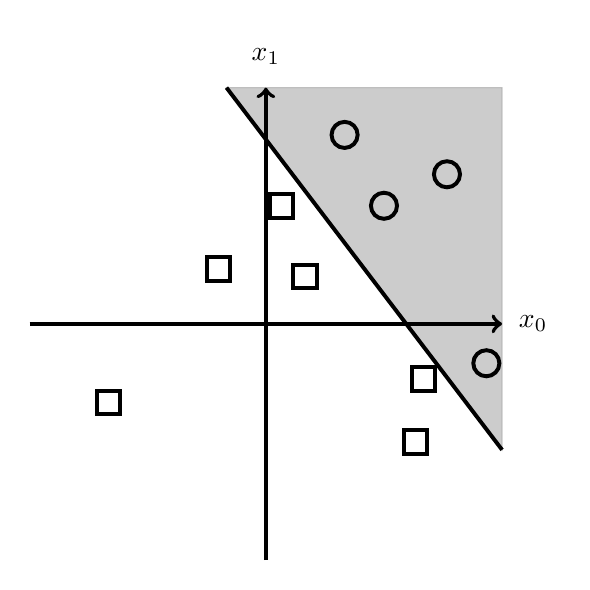
\begin{tikzpicture}[circle]
	
	\node (origin) at (0cm,0cm){};
	
	\draw[->,line width=0.5mm] (-3.0cm,0cm) -- (3.0cm,0cm)node[pos=1,right] {$x_0$};
	
	\draw[->,line width=0.5mm] (0cm,-3.0cm) -- (0cm,3.0cm)node[pos=1,above] {$x_1$};
	
	\node[circle,draw,line width=0.5mm,minimum size=0.3cm] at (2.3cm,1.9cm) {};
	\node[circle,draw,line width=0.5mm,minimum size=0.3cm] at (2.8cm,-0.5cm) {};
	\node[circle,draw,line width=0.5mm,minimum size=0.3cm] at (1.5cm,1.5cm) {};
	\node[circle,draw,line width=0.5mm,minimum size=0.3cm] at (1.0cm,2.4cm) {};
	
	\node[rectangle,draw,line width=0.5mm,minimum size=0.3cm] at (0.2cm,1.5cm) {};
	\node[rectangle,draw,line width=0.5mm,minimum size=0.3cm] at (-0.6cm,0.7cm) {};
	\node[rectangle,draw,line width=0.5mm,minimum size=0.3cm] at (-2cm,-1cm) {};
	\node[rectangle,draw,line width=0.5mm,minimum size=0.3cm] at (2cm,-0.7cm) {};
	\node[rectangle,draw,line width=0.5mm,minimum size=0.3cm] at (0.5cm,0.6cm) {};
	\node[rectangle,draw,line width=0.5mm,minimum size=0.3cm] at (1.9cm,-1.5cm) {};
	
	\coordinate (h1) at (3cm, -1.6cm);
	\coordinate (h2) at (-0.5, 3cm);
	%hipersík
	\draw[line width=0.5mm] (h1) -- (h2);
	
	\draw [fill=black, opacity=0.2]
	(h1) -- (h2) -- (3.0cm,3.0cm) -- cycle;
	
	\end{tikzpicture}
	\caption{Lineárisan szeparálható osztályozási feladat két bemeneti tulajdonsággal. Az egyik osztály \tikzcircle, a másik a \tikzrectangle. A vonal egy hipersík, melyhez tartozó perceptron helyesen oldja meg a feladatot}
\end{figure}

Természetesen nem minden feladat lineárisan szeparálható, sőt, a valós életben jelentkező feladatok jelentős része nem az. Az egyik legegyszerűbb példa a lineárisan nem szeparálható feladatra a XOR, ami a \aref{xor} ábrán látható.
\begin{figure}[H]
	\centering
	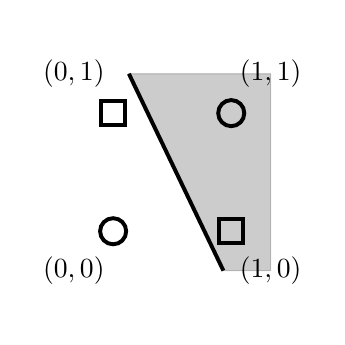
\begin{tikzpicture}[circle]
	
	\node (origin) at (0cm,0cm){};
	
	\node(bottomleft) [circle,draw,line width=0.5mm,minimum size=0.3cm] at (origin) {};
	
	\node(bottomleftlabel) at (-0.5cm,-0.5cm){$(0,0)$};
	
	\node(bottomright) [rectangle,draw,line width=0.5mm,minimum size=0.3cm] at (1.5cm,0cm) {};
	
	\node(bottomrightlabel) at (2cm,-0.5cm){$(1,0)$};
	
	\node(upperleft) [rectangle,draw,line width=0.5mm,minimum size=0.3cm] at (0,1.5cm) {};
	
	\node(upperleftlabel) at (-0.5cm,2cm){$(0,1)$};
	
	\node(topright) [circle,draw,line width=0.5mm,minimum size=0.3cm] at (1.5cm,1.5cm) {};
	
	\node(toprightlabel) at (2cm,2cm){$(1,1)$};
	
	\draw[line width=0.5mm] (0.2cm, 2cm) -- (1.4cm, -0.5cm);
	
	\draw [fill=black, opacity=0.2]
	(0.2cm, 2cm) -- (1.4cm, -0.5cm) -- (2cm,-0.5cm) -- (2cm,2cm) -- cycle;
	
	\end{tikzpicture}
	\caption{XOR feladat: négy tanító mintánk van, az egyik osztály a \tikzcircle, a másik a \tikzrectangle. A felrajzolt hipersík csak példa, a feladatot nem oldja meg}
	\label{xor}
\end{figure}

A működés tárgyalásából kimaradt a tanító algoritmus, mivel nem a Rosenblatt Perceptron a fejezet fókusza, ezáltal csak a modernebb hálózatok megértésében segítő részleteket érdemes tárgyalni.

\section{Több Rétegű Előrecsatolt Neurális Hálózatok}

Egy neurontól magától értetődő, hogy nem várhatjuk a komplexebb feladatok megoldását, hiszen a természetben is nagy számú neuron együttműködése szükséges ehhez, pedig az evolúció során nagy előny származott volna kompaktabb idegrendszerekből. 
Manapság a gyakorlatban több száz, esetenként sokezer neuront számláló hálózatok a megszokottak. Működésük megértéséhez először ismertetem az építőelemek főbb jellemzőit és az ehhez kapcsolódó terminológiát.

Ez a szekció csak az előrecsatolt neurális hálózatokat tárgyalja, ami azt jelenti hogy az információ folyamjukban nincs kör. Ennek oka, hogy visszacsatolt hálózatokat általában időben kiterjedt jelek feldolgozására használják, ami nem a dolgozat témája.

\newcommand{\y}{\ensuremath{\boldsymbol y}}
\newcommand{\yvesszo}{\ensuremath{\boldsymbol y'}}
\newcommand{\x}{\ensuremath{\boldsymbol x}}
\newcommand{\w}{\ensuremath{\boldsymbol w}}

\subsection{Neuron}
\label{neuron_section}
A Rosenblatt Perceptronnal foglalkozó fejezetben említettem, hogy a perceptron az egyetlen egy neuront szimbolizál. A modern értelemben vett neuronok azonban kicsit általánosabbak. A signum helyett más függvények is alkalmazhatók, ezeket aktivációs függvényeknek nevezzük.

\begin{figure}[H]
		\begin{subfigure}{\linewidth}
			\begin{tikzpicture}
                \begin{axis} [width=0.5\textwidth,samples=100,xmin=-3,xmax=3,xlabel=\yvesszo, ylabel=L,ymin=0, ymax=1]
                    \addplot[mark=none,line width=0.5mm] {(1/(1+e^(-x))};
                    \node at (-1.5,0.75) {$f(x) = \cfrac{1}{1+e^{-x}}$};
                \end{axis}
                
            \end{tikzpicture}
            \begin{tikzpicture}
                \begin{axis} [width=0.5\textwidth,samples=300,xmin=-1,xmax=1,xlabel=\yvesszo, ylabel=L,ymin=-0.1, ymax=1]
                    \addplot[mark=none,line width=0.5mm] {(x>0)*x};
                     \node at (-0.3,0.7) {$ f(x)=
                        \begin{cases}
                            0  &  \text{if } n<0\\
                            x  &  \text{if } n\geq0
                        \end{cases}$};
                \end{axis}
            \end{tikzpicture}
		\end{subfigure}
	\caption{Két gyakori aktivációs függvény. Baloldalon a sigmoid, jobboldalon a ReLu}
\end{figure}


Vannak speciális aktivációs függvények, például a softmax, amit a kimeneti neuronokon alkalmaznak és funkciója az, hogy a kimeneti vektort normalizálja, azaz a kimeneti értékek szummáját egyre állítja be és minden értéket a [0,1] intervallumra korlátoz. Ezzel ha a kimeneteket valószínűségként értelmezzük, azok egy teljes eseményrendszert alkotnak. Így minden kimenet értelmezhető úgy, hogy milyen valószínűséggel gondolja a hálózat, hogy a bemenet az adott osztályba tartozik.


A neuron tehát leírható a $y = f(\x^\intercal \w)$ kifejezéssel, ahol $x$ a bemenet, \w a súlyok $f$ pedig az aktivációs függvény. A Rosenblatt Perceptornnal ellentétben viszont az \x nem csak a háló bemenetét jelentheti, hanem más neuronok kimenetét is, hogy ehhez egységes jelölés rendszert lehessen kialakítani, be kell vezetni a rétegek fogalmát. A $\x^\intercal \w$ részeredményt szokás a neuron szummájának nevezni, és $s$ betűvel jelölni.
 
 
 
 \subsection{Rétegek}
 
Bár elméleti szempontból nem megkövetelt, de áttekinthetőségi és számítási komplexitás szempontjából a neurális hálózatokat rétegekre szokták osztani. Egy réteg általánosságban egy vagy több neuron olyan halmaza, amely ez előző réteg kimenetét tekinti bemenetének. Ez nem egy definíció, általában igaz, de vannak kivételek, például olyan hálózatok esetében, melyekben egy réteg több őt megelőzőt is felhasznál. Továbbá egy rétegbe tartozó neuronoknak jellemzően azonos az aktivációs függvénye. Elméleti szinten ez sincs megkövetelve, de számítási teljesítmény és implementációs komplexitás szempontjából előnyös.
Az $i$-edik réteg ($i = 1,2\dots, N$) kimenete legyen $\y^{(i)}$, a réteg $j$-edik ($j = 1,2\dots$)  neuronjának a kimenete pedig $y^{(i)}_j$. Értelemszerűen itt N a rétegek számát jelöli. Az i-edik réteg j-edik neuronjának súlyait tartalmazó vektor legyen $w^{(i)}_j$, az i-edik réteg minden neuronjának súlyait tartalmazó mátrix pedig $w^{(i)}$ (egy neuronhoz egy oszlop tartozik).   
 
\Aref{mlp} ábrán egy neurális hálózat látható, rajta feltüntetve a három réteg típus, amely minden több rétegű hálózatban megtalálható.
 
 A \emph{bemeneti réteg} az a réteg, ami a háló bemeneteit tartalmazza. A bemeneti tulajdonságokat szokás bemeneti neuronnak is nevezni, így fogalmilag egységesebb a reprezentáció. Ez mindig a hálózat első rétege, de esetenként több bemeneti réteget is lehet.
 
 A \emph{rejtett réteg} nevét arról kapta, hogy a külvilággal nem érintkezik, csak a hálózat többi rétegével. Ezen rétegek tetszés szerint konfigurálhatóak rétegek száma, neuronok  aktivációs függvénye, és a rétegek neuronszáma szempontjából.
 
 A \emph{kimeneti réteg} neuronjainak a kimenete az egész hálózat kimenete. Ez a réteg pontosan annyi neuront használ amennyi az elvárt kimenetek száma. Ez osztályozásnál gyakran az kategóriák száma. Ebben a rétegben leggyakrabban alkalmazott aktivációs függvény a softmax, amiről \aref{neuron_section} szekció említést tesz.

\begin{figure}[H]
    \centering
	\begin{tikzpicture}[circle]
	
		% inputs
		\node[line width=0.5mm,minimum size=0.5cm] (a) at (0cm,-0.25cm) {$x_0$};
		\node[line width=0.5mm,minimum size=0.5cm] (b) [below=0.3cm of a] {$x_1$};
		\node[line width=0.5mm,minimum size=0.5cm] (c) [below=0.3cm of b] {$x_2$};
		\node[line width=0.5mm,minimum size=0.5cm] (d) [below=0.3cm of c] {$x_3$};
		\node[line width=0.5mm,minimum size=0.5cm] (e) [below=0.3cm of d] {$x_4$};
		
		% first layer neurons 
		\node[line width=0.5mm,draw,minimum size=0.5cm,red] (aa) at (3cm,-0.85cm) {};
		\node[line width=0.5mm,draw,minimum size=0.5cm,green] (bb) [below=1.15cm of aa] {};
		\node[line width=0.5mm,draw,minimum size=0.5cm,blue] (cc) [below=1.15cm of bb] {};
		
		% second layer neurons 
		\node[line width=0.5mm,draw,minimum size=0.5cm] (aaa) at (6cm,-0.85cm) {};
		\node[line width=0.5mm,draw,minimum size=0.5cm] (bbb) [below=1.15cm of aaa] {};
		\node[line width=0.5mm,draw,minimum size=0.5cm] (ccc) [below=1.15cm of bbb] {};
		
		%output layer neuron
		\node[line width=0.5mm,draw,minimum size=0.5cm] (output) at (9cm,-2.55cm) {};

		
	    %connections to first layer
		\draw[line width=0.5mm,red] (a) -- (aa);
		\draw[line width=0.5mm,red] (b) -- (aa);
		\draw[line width=0.5mm,red] (c) -- (aa);
		\draw[line width=0.5mm,red] (d) -- (aa);
		\draw[line width=0.5mm,red] (e) -- (aa);
        
        \draw[line width=0.5mm,green] (a) -- (bb);
        \draw[line width=0.5mm,green] (b) -- (bb);
		\draw[line width=0.5mm,green] (c) -- (bb);
		\draw[line width=0.5mm,green] (d) -- (bb);
		\draw[line width=0.5mm,green] (e) -- (bb);
		
		\draw[line width=0.5mm,blue] (a) -- (cc);
		\draw[line width=0.5mm,blue] (b) -- (cc);
		\draw[line width=0.5mm,blue] (c) -- (cc);
		\draw[line width=0.5mm,blue] (d) -- (cc);
		\draw[line width=0.5mm,blue] (e) -- (cc);
		
		%connections to second layer
		\draw[line width=0.5mm,red] (aa) -- (aaa);
		\draw[line width=0.5mm,red] (aa) -- (bbb);
		\draw[line width=0.5mm,red] (aa) -- (ccc);
		
        \draw[line width=0.5mm,green] (bb) -- (aaa);
        \draw[line width=0.5mm,green] (bb) -- (bbb);
		\draw[line width=0.5mm,green] (bb) -- (ccc);
		
		\draw[line width=0.5mm,blue] (cc) -- (aaa);
		\draw[line width=0.5mm,blue] (cc) -- (bbb);
		\draw[line width=0.5mm,blue] (cc) -- (ccc);
		
		%conenctions to output layer
		\draw[line width=0.5mm] (aaa) -- (output);
		\draw[line width=0.5mm] (bbb) -- (output);
		\draw[line width=0.5mm] (ccc) -- (output);
		
		%output
		\node[right=1.5cm of output] (y) {y};
		\draw[->,line width=0.5mm] (output) -- (y);
		
		%input layer
		\draw[dashed,line width=0.5mm] (c) ellipse (0.7cm and 2.8cm);
		\node[above=1.8cm of c] {bemeneti réteg};
		
		%hidden layer 1
		\draw[dashed,line width=0.5mm] (bb) ellipse (0.6cm and 2.5cm);
		\node[above=1.3cm of bb] {rejtett réteg 1};
		
		%hidden layer 2
		\draw[dashed,line width=0.5mm] (bbb) ellipse (0.6cm and 2.5cm);
		\node[above=1.3cm of bbb] {rejtett réteg 2};
		
		%output layer
		\draw[dashed,line width=0.5mm] (output) ellipse (0.6cm and 1.5cm);
		\node[above=0.6cm of output] {kiemeneti réteg};
		
	\end{tikzpicture}
	\caption{Egy több rétegű neurális hálózat. A körök egy neuront jelentenek, az összeköttetések megmutatják, hogy melyik neuron honnan kap bemenetet. Az első rejtett réteg neuronjai az áttekinthetőség érdekében színezettek. \label{mlp}}
\end{figure}

A rejtett rétegeknek több típusa létezik:

\Aref{mlp} ábrán a rejtett rétegek \emph{sűrű kötésűek}, ami azt jelenti, hogy a réteg minden neuronjának bemenete az előző réteg összes kimenete. Ez a leggyakrabban alkalmazott réteg konfiguráció, de nem minden esetben a megfelelő döntés. A gyengesége, hogy a súlyok száma az előző és a tárgyalt réteg neuron számának a szorzata. Ez a négyzetes súlymennyiség előnytelenül nagy tanuló képességű hálózatot eredményez, ha valamelyik réteg nagy méretű. Ha ez olyan rétegnél lép fel, aminek a méretét nem tudjuk szabályozni, például a bemeneti réteg, akkor problémát jelenthet, mivel a kelleténél több paraméternek negatív hatása lehet (ezt egy későbbi szakaszban részletezem).

A \emph{lokális kötésű} réteg minden neuronja csak az előző réteg egy részhalmazát kapja bemenetként. Ezt egy csúszó ablak segítségével lehet egyszerűen megoldani, ami az előző rétegen csúsztatva egy neuronhoz az éppen az ablakba eső bemeneteket rendeli.

A mély neurális hálózatokban alkalmaznak még például konvolúciós és \foreignlanguage{english}{pooling} rétegeket is, ezekről a későbbiekben lesz szó.

\subsection{Hiba visszaterjesztés algoritmus}

A \foreignlanguage{english}{backpropagation}, vagy magyarul hiba visszaterjesztés algoritmus, ami már elméletben a '60-as években megszületett, de a neurális hálók terén a '80-as években terjedt el. A hiba visszaterjesztés ereje abban rejlik, hogy általánosan alkalmazható bármilyen neurális háló struktúrára,így egy lépéssel közelebb kerülünk a természetben lévő neurális hálókhoz.

Mielőtt magáról az algoritmusról beszélnénk be kell vezetni pár fogalmat. Ahhoz, hogy tanítani tudjunk meg kell fogalmazni egy célt. Ez tipikus esetben az, hogy a háló minden tanító példára pontosan az elvárt kimenetet adja vissza (az elvárt bemenet ezentúl legyen \y, a háló kimenete pedig \yvesszo). Ez önmagában még nem elegendő, mert nem mondja meg, hogyan érjük el azt a célt. A hibafüggvények azt adják meg, hogy mennyire jó egy megoldás, azáltal, hogy \y ~ és \yvesszo közti eltérés valamilyen függvényét képzik. Magától értetődő módon elvárt a hibafüggvényektől, hogy tökéletes megoldás esetén a globális minimumukat vegyék fel, ez gyakran a nulla, bár ez elméleti szempontból nem megkövetelt. Másik fontos elvárás, hogy csak egy minimum pont legyen, különben gradiensre alapuló iteratív algoritmusok beragadhatnak lokális minimumokba. 
Több különböző hibafüggvény alkalmaznak a gyakorlatban, két példa megtekinthető \aref{loss} ábrán.

\begin{figure}[H]
		\begin{subfigure}{\linewidth}
			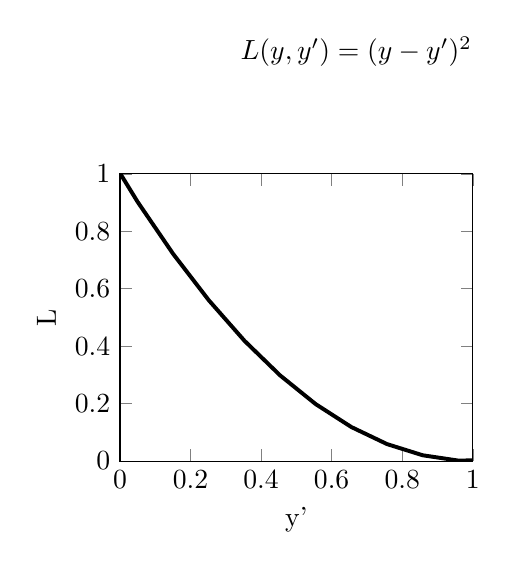
\begin{tikzpicture}
                \begin{axis} [width=0.5\textwidth,samples=100,xmin=0,xmax=1,xlabel=y', ylabel=L,ymin=0, ymax=1]
                    \addplot[mark=none,line width=0.5mm] {(1-x)^2};
                \end{axis}
                \node at (3,5.2) {$L(y,y') = (y - y')^2$};
            \end{tikzpicture}
            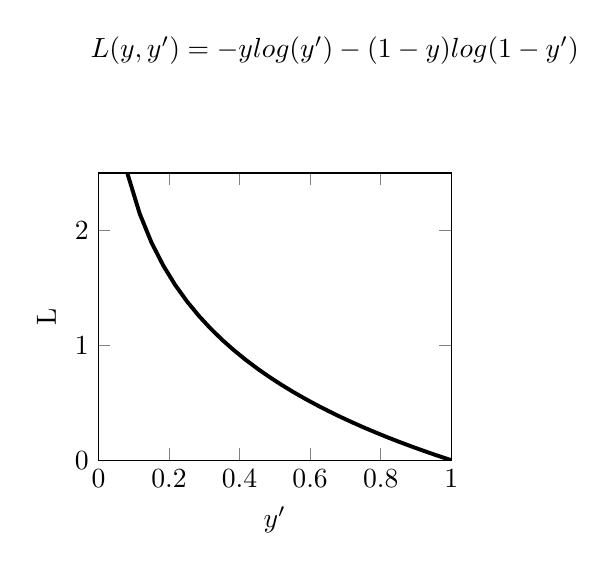
\begin{tikzpicture}
                \begin{axis} [width=0.5\textwidth,samples=300,xmin=0,xmax=1,xlabel=\yvesszo, ylabel=L,ymin=0, ymax=2.5]
                    \addplot[mark=none,line width=0.5mm] {-ln(x)};
                \end{axis}
                \node at (3,5.2) {$L(y,y') = -y log(y') - (1-y) log(1-y')$};
            \end{tikzpicture}
		\end{subfigure}
	\caption{Két gyakori hiba függvény grafikonja $y=1$ esetben. Baloldalt a négyzetes hiba, jobboldalt a keresztentrópia. Megfigyelhető hogy mindkettő akkor veszi fel a nulla értéket ha $y = y'$ \label{loss}.}
\end{figure}
	
A hiba visszaterjesztés úgy tanítja a hálót, hogy annak minden szabad paramétere szerint meghatározza egy hibafüggvény deriváltját, majd ezt egy tanulási sebesség (vagy bátorsági tényező) nevezetű konstanssal megszorozva kivonja a paraméter értékéből, így a paraméterek egy olyan állapotát létrehozva, ami a hibafüggvény értékét csökkenti.

A pontos működés megértéséhez formálisan is meg kell fogalmaznunk az algoritmust. Erre talán a legszemléletesebb út egy példán keresztül vezet.

Használjuk \aref{mlp} ábrán látható hálózati struktúrát példaként, feltételezve, hogy minden neuron aktivációs függvénye szigmoid és a hibafüggvény a négyzetes hiba.
A példa hálózat speciális abból a szempontból, hogy kimeneti rétege egy neuronból áll. Általános esetben a kimenet egy vektor lenne, ami az kimeneti réteg neuronjainak kimenetéből állna.  Az egyszerűség kedvéért egy elemű vektor helyett skalárként kezelem a kimenetet. Továbbá a kimeneti réteg függvényét a réteg indexe nélkül használom annak ellenére, hogy a jelölési konzisztencia megkövetelné, hogy éreztessem, hogy az a teljes háló kimenete.


\begin{equation}
    y(x) = f^{(4)}\left(s^{(4)}_1\right) = \cfrac{1}{1+e^{-(s^{(4)}_1)}} = \cfrac{1}{1+e^{-(\y^{\intercal \sm{(3)}}\w^{\sm{(4)}}_1)}}
\end{equation}

\begin{equation}
    y^{\sm{(3)}}\left(x\right) =
    \begin{bmatrix}
    f^{\sm{(3)}}\left(s^{(3)}_1\right) \\
    f^{\sm{(3)}}\left(s^{(3)}_2\right) \\
    f^{\sm{(3)}}\left(s^{(3)}_3\right)
    \end{bmatrix}
     = 
    \begin{bmatrix}
    f^{(\sm{3)}}\left(\y^{\intercal(\sm{2})}*\w^{(3)}_1\right) \\
    f^{(\sm{3})}\left(\y^{\intercal(\sm{2})}*\w^{(3)}_2\right) \\
    f^{(\sm{3})}\left(\y^{\intercal(\sm{2})}*\w^{(3)}_3\right)
    \end{bmatrix}
    \label{outputlayer}
\end{equation}
\begin{equation}
    y^{\sm{(2)}}\left(x\right) =
    \begin{bmatrix}
    f^{(\sm{2)}}\left(\y^{\intercal(\sm{1})}*\w^{(2)}_1\right) \\
    f^{(\sm{2})}\left(\y^{\intercal(\sm{1})}*\w^{(2)}_2\right) \\
    f^{(\sm{2})}\left(\y^{\intercal(\sm{1})}*\w^{(2)}_3\right)
    \end{bmatrix}
\end{equation}

\begin{equation}
    y^{\sm{(1)}}\left(x\right) = \x
\end{equation}

%TODO az y és y' jelölés konzisztensé tétele, a kimenet legyen y az elvárt kimenet meg valami y^{exp}

Látható, hogy minden réteg kimenetének számítása egy kaptafára megy, a kimeneti réteg is legfőképpen külalakilag különbözik, mivel ott behelyettesítettem az aktivációs függvénnyel. Ez a moduláris számíthatóság teszi lehetővé tetszőleges méretű háló létrehozását.

Megfigyelhető, hogy minden réteg csak az őt megelőző bemenetétől függ (kivéve a bemeneti réteg), ezért a hálózat kiszámítását az elején kell kezdeni, így szokták \foreignlanguage{english}{forward pass}-nak is nevezni.

A háló függvényének ismeretében, rátérhetünk annak deriválására. Mivel célunk egy súly szerint parciálisan deriválni, be kell vezetni egy jelölést rá, $\w^{\sm{(n)}}_{i,j}$ legyen az $n$-edik réteg $i$-edik neuronjának $j$-edik súlya. Jelöljük a hibafüggvényt $L(\yvesszo,\y)$-el, továbbá ennek a $w^{(n)}_{i,j}$ súly szerinti deriváltját jelöljük Leibniz jelöléssel  a $\cfrac{\partial L}{\partial w^{(n)}_{i,j}}$ kifejezésként.  
 

Felhasználható a $f(g(x))' = f'(g(x))*g'(x)$ deriválási szabály, ami jelen esetben ekvivalens a $\cfrac{\partial f}{\partial x} =  \cfrac{\partial f}{\partial g}~ \cfrac{\partial g}{\partial x}$ kifejezéssel.
Először keressük meg a hibafüggvény $w^{(4)}_{1~1}$  súly szerinti deriváltját.

\begin{equation}
    \cfrac{\partial L}{\partial w^{(4)}_{1,1}} = \cfrac{\partial L}{\partial y'}~ \cfrac{\partial y'}{\partial w^{(4)}_{1,1}} = \cfrac{\partial L}{\partial y'}~ \cfrac{\partial y'}{\partial f^{(4)}}~\cfrac{\partial f^{(4)}}{\partial w^{(4)}_{1,1}} = \cfrac{\partial L}{\partial y'}~\cfrac{\partial y'}{\partial f^{(4)}}~\cfrac{\partial f^{(4)}}{\partial s^{(4)}_{1}}~\cfrac{\partial s^{(4)}_{1}}{\partial w^{(4)}_{1,1}}
    \label{derivoutputlayer}
\end{equation}

A láncszabály segítségével sikerült felbontani a feladatot négy egyszerűbb feladat szorzatára, amik önmagukban megoldhatóak.

\begin{equation}
    \cfrac{\partial L}{\partial y'} = \cfrac{\partial}{\partial y'}(y-y')^2= -2(y-y') 
\end{equation}

Megjegyezendő, hogy itt y az elvárt kimenet, ami konstans. Könnyen összetéveszthető y és y', mivel y(x) a háló függvénye miközben a kimenetét y'-nek hívjuk. 

\begin{equation}
    \cfrac{\partial y'}{\partial f^{(4)}} = 1
\end{equation}

Ez a tag azért 1, mert az y(x) függvény lényegében csak egy alias a kimeneti neuron aktivációjának kimenetére ezért egyenlete effektíve $y(x) = 1*f^{(4)}(x)$. A továbbiakban összevonva szerepel a két függvény y' jelöléssel.

\begin{equation}
    \cfrac{\partial f^{(4)}}{\partial s^{(4)}_{1}} = \cfrac {\partial}{\partial  s^{(4)}_{1}} \cfrac{1}{1+e^{- s^{(4)}_{1}}} = \cfrac{1}{1+e^{-s^{(4)}_{1}}}* \left(1 - \cfrac{1}{1+e^{-s^{(4)}_{1}}}\right)
\end{equation}

Ez a tényező adja meg az aktivációs függvény szerinti deriváltat, melynek egyenletéről első pillantásra igen nehéz megmondani az alakját, ezt \aref{sigderiv} ábra szemlélteti.

 \begin{figure}[H]
        \centering
		\begin{tikzpicture}
            \begin{axis} [width=0.7\textwidth,height=0.5\textwidth,samples=100,xmin=-4,xmax=4,xlabel=x, ylabel=f,ymin=0, ymax=0.5]
                \addplot[mark=none,line width=0.5mm] {(1/(1+e^(-x))*(1-1/(1+e^(-x)))};
            \end{axis}
            \node at (4.5,4.6) {$f'(x) = \left(\cfrac{1}{1+e^{-x}}\right)' = \cfrac{1}{1+e^{-x}} \left(1 - \cfrac{1}{1+e^{-x}}\right)$};
        \end{tikzpicture}
	\caption{A sigmoid aktivációs függvény deriváltja \label{sigderiv}}
\end{figure}

\begin{equation}
    \cfrac{\partial s^{(4)}_{1}}{\partial w^{(4)}_{1~1}} = \cfrac{\partial }{\partial w^{(4)}_{1~1}} \yvesszo^{(3) \intercal}* \w^{(4)}_1= \cfrac{\partial }{\partial w^{(4)}_{1~1}}~ w^{(4)}_{1~1}y^{(3)}_{1} + w^{(4)}_{1~2}y^{(3)}_{2} + w^{(4)}_{1~4}y^{(3)}_{3} = y^{(3)}_{1}
    \label{weightderiv}
\end{equation}

Látható, hogy \aref{derivoutputlayer} egyenletben azért nem volt szükség tovább bontani a problémát, mivel az a tag tartalmazza a súlyt ami szerint deriválunk. Szerencsénkre az, hogy sok tag van nem nehezíti a számolást, mivel egy tagon kívül mindegyik konstansnak számít és kiesik.

Az ismeretett kifejezések szorzata megadja a hálózat  $w^{(4)}_{1~1}$ súly szerinti deriváltját, de könnyen látható hogy csupán az indexek megváltoztatásával a kimeneti réteg bármely súlyára alkalmazhatók ezen egyenletek. A harmadik réteg súlyainak deriváltja a kimeneti réteghez hasonló módon számítható. Legyen most a keresett derivált $\cfrac{\partial L}{\partial w^{(3)}_{1~1}}$.

\begin{equation}
    \cfrac{\partial L}{\partial w^{(3)}_{1~1}} = \cfrac{\partial L}{\partial s^{(4)}_{1}}~\cfrac{\partial s^{(4)}_{1}}{\partial  w^{(3)}_{1~1}} = \cfrac{\partial L}{\partial s^{(4)}_{1}}~\cfrac{\partial s^{(4)}_{1}}{\partial y^{(3)}_1}~\cfrac{\partial y^{(3)}_1}{\partial  w^{(3)}_{1~1}} = 
    \cfrac{\partial L}{\partial s^{(4)}_{1}}~\cfrac{\partial s^{(4)}_{1}}{\partial y^{(3)}_1}~\cfrac{\partial y^{(3)}_1}{\partial f^{(3)}}~\cfrac{\partial f^{(3)}}{\partial s^{(3)}_{1}}~\cfrac{\partial s^{(3)}_{1}}{\partial  w^{(3)}_{1~1}}
    \label{derivthirdlayer}
\end{equation}
%valahova említés aktiváció vetkort kap jelölésről

A $\cfrac{\partial L}{\partial s^{(4)}_{1}}$ deriváltat egy kifejezésként jelöltem, mivel felbontása fentebb már ismertetett. Látható, hogy az utolsó három tag is analóg a kimeneti rétegben kiszámoltakhoz, $\cfrac{\partial s^{(4)}_{1}}{\partial y^{(3)}_1}$ tag az egyetlen ami még nem szerepelt.

\begin{equation}
    \cfrac{\partial s^{(4)}_{1}}{\partial y^{(3)}_1} = \cfrac{\partial }{\partial y^{(3)}_1}~\y^{(3)\intercal} \w^{(4)}_1 =\cfrac{\partial }{\partial y^{(3)}}~ w^{(4)}_{1~1}y^{(3)}_{1} + w^{(4)}_{1~2}y^{(3)}_{2} + w^{(4)}_{1~4}y^{(3)}_{3} = w^{(4)}_{1~1}
\end{equation}

Ennek kiszámításához viszont egy speciális körülmény is fel lett használva. Általános esetben a $\cfrac{\partial L}{\partial s^{(4)}_{1}}$ nem használható mivel, nem csak a $ s^{(4)}_{1}$ függ $w^{(3)}_{1~1}$ súlytól, hanem a 4-es indexű réteg minden szummája. Mivel jelen esetben ez a 4-es réteg csak egy neuronból áll, a két kifejezés ekvivalens. Tekintsük viszont $w^{(2)}_{1~1}$-es súlyt, feltételezve, hogy a harmadik réteg szummáinak deriváltjai már ismertek, tehát tudjuk $\cfrac{\partial L}{\partial s^{(3)}_1}$,$\cfrac{\partial L}{\partial s^{(3)}_2}$ és $\cfrac{\partial L}{\partial s^{(3)}_3}$ értékét. Ekkor amire szükség van az a $\cfrac{\partial s^{(3)}_1}{\partial w^{(2)}_{1~1}}$, $\cfrac{\partial s^{(3)}_2}{\partial w^{(2)}_{1~1}}$ és $\cfrac{\partial s^{(3)}_3}{\partial w^{(2)}_{1~1}}$.

\begin{subequations}
    \begin{equation}
        \cfrac{\partial s^{(3)}_1}{\partial w^{(2)}_{1~1}} = \cfrac{\partial s^{(3)}_1}{\partial y^{(2)}_1}~\cfrac{\partial y^{(2)}_1}{\partial s^{(2)}_1}~\cfrac{\partial s^{(2)}_1}{\partial w^{(2)}_{1~1}}
    \end{equation}    
    \begin{equation}
        \cfrac{\partial s^{(3)}_2}{\partial w^{(2)}_{1~1}} = \cfrac{\partial s^{(3)}_2}{\partial y^{(2)}_1}~\cfrac{\partial y^{(2)}_1}{\partial s^{(2)}_1}~\cfrac{\partial s^{(2)}_1}{\partial w^{(2)}_{1~1}}
    \end{equation}
    \begin{equation}
        \cfrac{\partial s^{(3)}_3}{\partial w^{(2)}_{1~1}} = \cfrac{\partial s^{(3)}_3}{\partial y^{(2)}_1}~\cfrac{\partial y^{(2)}_1}{\partial s^{(2)}_1}~\cfrac{\partial s^{(2)}_1}{\partial w^{(2)}_{1~1}}
    \end{equation}
\end{subequations}

Az L szerinti derivált számításához ezt a három komponenst összegezni kell, hiszen ezek tulajdonképpen a derivált függvény ágai, melyek a kimeneti neuron szummájánál ágaztak el, mivel annak minden komponense függ $w^{(2)}_{1~1}$ súlytól. A derivált ezen elágazását szemlélteti \aref{w221} ábra.

A hiba függvény $w^{(2)}_{1~1}$ súly szerinti deriváltja a következő réteg deriváltjainak ismeretében tehát:

\begin{equation}
    \cfrac{\partial L}{\partial w^{(2)}_{1~1}} = \left(\cfrac{\partial L}{\partial s^{(3)}_1}\cfrac{\partial s^{(3)}_1}{\partial y^{(2)}_1} + \cfrac{\partial L}{\partial s^{(3)}_2}\cfrac{\partial s^{(3)}_2}{\partial y^{(2)}_1} +\cfrac{\partial L}{\partial s^{(3)}_3} \cfrac{\partial s^{(3)}_3}{\partial y^{(2)}_1}\right)\cfrac{\partial y^{(2)}_1}{\partial s^{(2)}_1}~\cfrac{\partial s^{(2)}_1}{\partial w^{(2)}_{1~1}} 
\end{equation}

\begin{figure}[H]
    \centering
	\begin{tikzpicture}[circle]
	    % inputs
		\node[line width=0.5mm,minimum size=0.5cm,opacity=0.2] (a) at (0cm,-0.25cm) {$x_0$};
		\node[line width=0.5mm,minimum size=0.5cm,opacity=0.2] (b) [below=0.3cm of a] {$x_1$};
		\node[line width=0.5mm,minimum size=0.5cm,opacity=0.2] (c) [below=0.3cm of b] {$x_2$};
		\node[line width=0.5mm,minimum size=0.5cm,opacity=0.2] (d) [below=0.3cm of c] {$x_3$};
		\node[line width=0.5mm,minimum size=0.5cm,opacity=0.2] (e) [below=0.3cm of d] {$x_4$};
	
		% first layer neurons 
		\node[line width=0.5mm,draw,minimum size=0.5cm] (aa) at (3cm,-0.85cm) {};
		\node[line width=0.5mm,draw,minimum size=0.5cm,opacity=0.2] (bb) [below=1.15cm of aa] {};
		\node[line width=0.5mm,draw,minimum size=0.5cm,opacity=0.2] (cc) [below=1.15cm of bb] {};
		
		% second layer neurons 
		\node[line width=0.5mm,draw,minimum size=0.5cm] (aaa) at (6cm,-0.85cm) {};
		\node[line width=0.5mm,draw,minimum size=0.5cm] (bbb) [below=1.15cm of aaa] {};
		\node[line width=0.5mm,draw,minimum size=0.5cm] (ccc) [below=1.15cm of bbb] {};
		
		%output layer neuron
		\node[line width=0.5mm,draw,minimum size=0.5cm] (output) at (9cm,-2.55cm) {};
		
		%connections to first layer
		\draw[line width=0.5mm,opacity=0.2] (a) -- (aa);
		\draw[line width=0.5mm,opacity=0.2] (b) -- (aa);
		\draw[line width=0.5mm,opacity=0.2] (c) -- (aa);
		\draw[line width=0.5mm,opacity=0.2] (d) -- (aa);
		\draw[line width=0.5mm,opacity=0.2] (e) -- (aa);
        
        \draw[line width=0.5mm,opacity=0.2] (a) -- (bb);
        \draw[line width=0.5mm,opacity=0.2] (b) -- (bb);
		\draw[line width=0.5mm,opacity=0.2] (c) -- (bb);
		\draw[line width=0.5mm,opacity=0.2] (d) -- (bb);
		\draw[line width=0.5mm,opacity=0.2] (e) -- (bb);
		
		\draw[line width=0.5mm,opacity=0.2] (a) -- (cc);
		\draw[line width=0.5mm,opacity=0.2] (b) -- (cc);
		\draw[line width=0.5mm,opacity=0.2] (c) -- (cc);
		\draw[line width=0.5mm,opacity=0.2] (d) -- (cc);
		\draw[line width=0.5mm,opacity=0.2] (e) -- (cc);
		
		%connections to second layer
		\draw[line width=0.5mm] (aa) -- (aaa);
		\draw[line width=0.5mm] (aa) -- (bbb);
		\draw[line width=0.5mm] (aa) -- (ccc);
		
        \draw[line width=0.5mm,opacity=0.2] (bb) -- (aaa);
        \draw[line width=0.5mm,opacity=0.2] (bb) -- (bbb);
		\draw[line width=0.5mm,opacity=0.2] (bb) -- (ccc);
		
		\draw[line width=0.5mm,opacity=0.2] (cc) -- (aaa);
		\draw[line width=0.5mm,opacity=0.2] (cc) -- (bbb);
		\draw[line width=0.5mm,opacity=0.2] (cc) -- (ccc);
		
		%conenctions to output layer
		\draw[line width=0.5mm] (aaa) -- (output);
		\draw[line width=0.5mm] (bbb) -- (output);
		\draw[line width=0.5mm] (ccc) -- (output);
		
		%output
		\node[right=1.5cm of output] (y) {y};
		\draw[->,line width=0.5mm] (output) -- (y);
		
		%hidden layer 1
		\node[above=1.3cm of bb] {réteg 2};
		
		%hidden layer 2
		\node[above=1.3cm of bbb] {réteg 3};
		
		%output layer
		\node[above=0.6cm of output] {réteg 4};
		
	\end{tikzpicture}
	\caption{a hálózat struktúrája, kiemelve azok a neuronok és súlyokat reprezentáló vonalak, melyek függenek $w^{(2)}_{1~1}$ súlytól \label{w221}}
\end{figure}

A példa alapján egyszerűen felírható általánosságban a hibavisszaterjesztés algoritmus a n-edik réteg i-edik neuronjának j-edik súlyára, feltételezve hogy a következő réteg deriváltjai már ismertek és az n+1-es indexű réteg K darab neuront tartalmaz:

\begin{equation}
    \cfrac{\partial L}{\partial w^{(n)}_{i~j}} = \sum^{K}_{k=1} \left(\cfrac{\partial L}{\partial s^{(n+1)}_k}~\cfrac{\partial s^{(n+1)}_k}{\partial y^{(n)}_i}\right) \cfrac{\partial y^{(n)}_i}{\partial s^{(n)}_i}~\cfrac{\partial s^{(n)}_i}{\partial w^{(n)}_{i~j}} 
\end{equation}

Megfigyelhető, hogy minden réteg esetében a következő réteg deriváltjaira van szükség, ezért a derivált számítást a kimeneti rétegtől visszafelé kell számítani. Ezt a műveletet ezért backpass-nak nevezik és az algoritmus és erről kapta a nevét.

%TODO epochok
\subsection{Epochok}

\subsection{Súlyok frissítése}

Miután megvan a gradiens vektorunk minden súlyra, segítségével valahogy módosítanunk kell értéküket. A gradiens vektor csak azt mutatja meg, hogy a jelenlegi állapot végtelen kicsi környezetében merre csökken a hibafüggvény. Ezáltal ha túl nagyot lépünk, akkor lehet hogy egy olyan állapotba kerülünk ami már túlugrott az alacsonyabb területen és nagyobb hibát ad. Ha túl kicsire állítjuk a lépést, akkor nagyon lassú lesz a tanulás és könnyebben beragadhat lokális minimumokba.

A megfelelő tanítási sebesség feladatfüggő és a többi hiperparaméter is befolyásolhatja. Például nagyobb batch-méretnél - amiről a következő szekcióban lesz szó - nagyobb tanítási sebesség indokolt, mert a gradiens vektor hossza általában kisebb lesz. 

Ha a háló átlagos hibáját az epochok szerint ábrázoljuk és azt tapasztaljuk, hogy a grafikon egy ponton ellaposodik és nem változik tovább, valószínűleg túl kicsi a tanulási sebesség. Ha a globális minimumban állt meg a tanulás, akkor is ilyen formájú grafikont kapunk tehát ez nem minden esetben probléma. Ha folyamatosan emelkedik és esetleg be is áll egy nagyon magas értékre, akkor túl nagy a tanítási sebesség, amitől a súlyok divergáltak.  

\begin{figure}[H]
		\begin{subfigure}{\linewidth}
			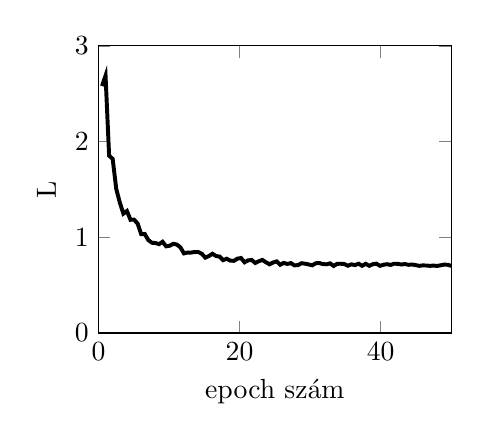
\begin{tikzpicture}
                \begin{axis} [width=0.5\textwidth,samples=100,xmin=0,xmax=50,xlabel=epoch szám, ylabel=L,ymin=0, ymax=3,domain=0:50]
                    \addplot[mark=none,line width=0.5mm] {max(1/(x/3+0.5),0.1)+(rnd/(x))+0.6};
                \end{axis}
                %\node at (3,5.2) {$L(y,y') = (y - y')^2$};
            \end{tikzpicture}
            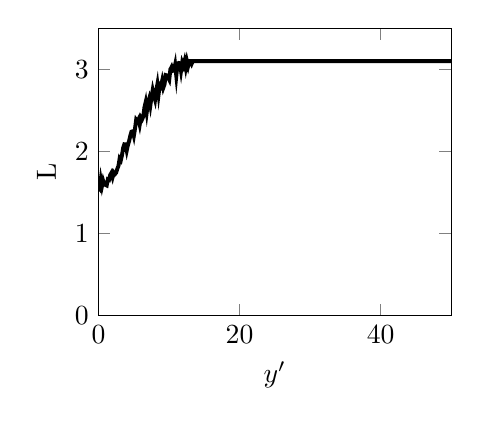
\begin{tikzpicture}
                \begin{axis} [width=0.5\textwidth,samples=300,xmin=0,xmax=50,xlabel=\yvesszo, ylabel=L,ymin=0, ymax=3.5,domain=0:50]
                    \addplot[mark=none,line width=0.5mm] {min(3.5-1/((x/10)^2+0.5)+rnd/6,3.1)};
                \end{axis}
                %\node at (3,5.2) {$L(y,y') = -y log(y') - (1-y) log(1-y')$};
            \end{tikzpicture}
		\end{subfigure}
	\caption{Tanulási sebességből adódó problémák. Bal oldalon a túl kis sebességből adódó ellaposodás, jobb oldalon pedig a divergencia.  \label{divergence}}
\end{figure}

\section{Batch tanítás}

A korábban ismertetett hibafüggvények egy tanítómintára számították a hibát, viszont a gyakorlatban szokás több mintát felhasználó hibafüggvényeket használni. Például az átlagos négyzetes hiba
\begin{equation}
    f(x) = \cfrac{1}{N}\sum^{N}_{i=1} (\y_i-\y^{exp}_i)^2,
\end{equation}
ahol N a \emph{batch méret} és \y az N darab tanítópéldára adott kimenetet tartalmazó vektor, $\y^{exp}$ pedig az ezekhez tartozó elvárt kimenetek vektora.

A batch tanítás több előnnyel is jár:
\begin{itemize}
    \item A deriváltak nagyságának kiegyenlítése. Egy tanítópélda esetén lehet, hogy bizonyos súlyokhoz nagyon nagy derivált rendelődik, ami miatt könnyebben divergálhat a tanulás. Tanulási sebesség levétele pedig azt eredményezné, hogy amelyik súlyokon kicsi a derivált, azok szinte nem változnak. Ha egyszerre sok példát használunk, akkor általánosságban tapasztalható, hogy ezen nagy gradiensek kiátlagolódnak egy egyenletesebbé.
    \item Gyorsítja a tanítást. Batch tanítás nélkül egy forward passhoz egy backward pass tartozik és a backward pass megváltoztatja a hálót ezért a következő forward passal nem párhuzamosítható. Viszont batch tanításnál N darab forward pass és aztán 1 db backward pass történik, ezen forward passok párhuzamosíthatóak, ezáltál a modern masszívan párhuzamosított hardware eszközökön nagyságrendekkel jobb tanítási sebesség érhető el.
    \item Segít elkerülni a túltanulást. Ha a háló egyszerre sok példát kap, akkor abban a gradiensben erősebb lesz az általános, legtöbb példára igaz összefüggés, ezáltal a véletlen zajok gradiensei kioltják egymást. 
\end{itemize}

Az optimális batch méret minden felhasználási esetben eltér. Ökölszabályként gyakran használt a 128-as batch méret, de gyakran nem ez a legmegfelelőbb. Fontos viszont, hogy a tanító adathalmaz legalább egy pár batchet fel tudjon tölteni, mivel ha csak egy batch van, akkor nagy eséllyel lokális minimumba ragadhat a tanítás, ha egy helyen közel nulla gradienst kapunk, vagy egy "völgy" két partján oszcillál. Viszont ha több batch van, akkor annak az esélye, hogy mindegyiknél az állapottér ugyanabban a pontjában van lokális minimum sokkal kisebb.

\section{Bemeneti attribútumok}
A bemeneti réteg neuronjait csak a terminológiai egyszerűség végett nevezik neuronnak, valójában minden neuron a bemeneti tulajdonságokat tartalmazó $\boldsymbol x$ vektor eleme. Ezen bemenetek lehetnek folytonos értékűek (pl. hőmérséklet), diszkrétek, ezen belül nem korlátos értékkészletűek (pl. életkor), illetve korlátosak (pl. digitális pixel intenzitás).
\subsection{One-Hot kódolás}
A véges számú állapotot felvevő attribútumok lehetnek kategorikusak, például az ország. Ez a megkülönböztetés azért fontos, mert ha például Magyarországot 0 kóddal látjuk el, Angliát 1-el és Svájcot 2-vel, az nem azt jelenti, hogy Magyarország és Anglia hasonlóbb, mint Magyarország és Svájc annak ellenére, hogy a szimpla numerikus értékek erre utalnak. Ekkor hogy a háló számára egyszerűbben "értelmezhető" legyen a bemenet, érdemes lehet alkalmazni a one-hot kódolást.

A módszer lényege, hogy a tulajdonság minden értékének egy új bemenetet veszünk fel, ami csak akkor vesz fel 1 értéket, mikor az eredeti tulajdonság a a hozzá tartozó értéket vette fel. Lényegében egy N értéket felvevő tulajdonságból lesz N tulajdonság, amiből egyszerre pontosan egy aktív.

A módszer segítségével a hálónak nincs szüksége extra logikát kialakítani ahhoz, hogy Svájcot ne egy kétszer olyan erős Angliának értelmezze, ezzel gyorsítva a tanulást. Viszont hátránya is van a módszernek: Nagyban növeli a bemenetek számát, ezzel könnyítve az overfitting megjelentését, ezáltal, mérlegelni kell, hogy bizonyos esetekben érdemesebb-e kihagyni a tulajdonságot a bemenetből. A kihagyás azért is mérlegelendő, mivel ahhoz, hogy összefüggést találjon a háló nagyon sok értéket felvevő kategorikus tulajdonságok közt, sok tanító példára van szükség, ha ez nincs jelen, nem valószínű hogy a tulajdonság jelenléte jelentős hozzájárulást jelentene a tanuláshoz.
\begin{figure}[H]
	{\tabcolsep=0pt\def\arraystretch{1.3}
		\begin{center}
			\begin{tabular}{ x{3cm}|x{1cm}|x{1cm}|x{1cm} }
				Eredeti kódolás & \multicolumn{3}{c}{One-hot kódolás} \tabularnewline
				\hline
				$x_0$ & $x_0$ & $x_1$  & $x_2$ \tabularnewline
				\hline
				0 & 1 & 0  & 0 \tabularnewline
				\hline
				1 & 0 & 1  & 0 \tabularnewline  
				\hline
				2 & 0 & 0  & 1 \tabularnewline    
			\end{tabular}
	\end{center}}
\end{figure}
%TODO ez az egész
\section{Mély neurális hálók}

\subsection{Új hálózati elemek}

Két új jelentős réteg típus  használatos a mély neurális hálókban.
\subsubsection{Konvolúciós réteg}



\subsection{Felhasználási területek}
